\documentclass[11pt,a4paper]{article}
\usepackage[margin=23mm]{geometry}
\usepackage[T1]{fontenc}
\usepackage{lmodern,microtype,amsmath,amssymb,booktabs,graphicx,siunitx}
\usepackage[colorlinks=true,linkcolor=blue,urlcolor=blue,citecolor=blue]{hyperref}
\setlength{\parskip}{0.35em}
\setlength{\parindent}{0pt}
\setlength{\emergencystretch}{2em}
\newcommand{\CrossTime}{0.1024}
\newcommand{\ReferenceFlux}{1.7244e+05}
\newcommand{\ReferenceHeat}{2.7634e+05}
\newcommand{\PerfectExcess}{30.666}
\newcommand{\DenseError}{2.8422e-13}
\newcommand{\BalanceError}{0.0018219}
\newcommand{\DomainError}{7.0024e-13}
\newcommand{\FinalOrder}{2.0049}
\newcommand{\SmoothOrder}{1.9998}

\title{ContactScale: resolving thermal contact\protect\\before diffusion hides it}
\author{}
\date{Computational study, 19 October 2026}
\begin{document}
\maketitle
\vspace{-2em}
\begin{abstract}
Can an accurate late-time heat flux conceal an unresolved initial contact?
This reproducible study compares a conservative finite-volume chain with a
semi-infinite analytical solution for two solids separated by a constant thermal
contact resistance. Modal propagation removes time-stepping error from the
comparison. For independently chosen synthetic properties, flux convergence at
one second approaches order \FinalOrder, yet even the finest tested mesh retains
a substantial initial flux deficit. The difference follows directly from the
half-cell thermal resistances. Analytical limits, an independent matrix
exponential, a surface-impedance integral and separate domain and smooth-solution
checks distinguish algebraic, spatial and model errors. These are verification
experiments, not physical validation or a claim of a new heat-transfer law.
\end{abstract}

\section{Research question and continuum model}
Contact resistance introduces an early response scale that a mesh can fail to
resolve even when a later temperature or flux appears converged. The question is
how to expose this mismatch without confusing it with time-integration error.
The study is motivated by thermal resistance, effusivity and interface
reconstruction in DTU MMME lectures 2--4, inspected read-only. All code, text,
parameters and figures here are original; no course data or solutions are used.

Consider one-dimensional conduction on each side of a stationary interface:
\begin{equation}
 c_i\partial_t T_i=k_i\partial_{xx}T_i,\qquad
 q=-k_L T_{L,x}(0^-,t)=-k_R T_{R,x}(0^+,t),\qquad
 T_L(0^-,t)-T_R(0^+,t)=Rq. \label{eq:pde}
\end{equation}
Here $c_i$ is volumetric heat capacity, $k_i$ conductivity and $R$ area-specific
contact resistance. Initially each half-space has a uniform temperature, with
gap $\Delta=T_{L,0}-T_{R,0}>0$. Properties and $R$ are constant; there is no
interfacial storage, radiation, phase change, convection or mechanical coupling.

Set $e_i=\sqrt{k_ic_i}$ and $b=e_L^{-1}+e_R^{-1}$. The half-space surface
impedances give, in the Laplace variable $s$,
\begin{equation}
 \widehat q(s)=\frac{\Delta}{Rs+b\sqrt{s}},\qquad
 q(t)=\frac{\Delta}{R}\operatorname{erfcx}(z),\quad
 z=\frac{b\sqrt t}{R},\quad t_c=(R/b)^2. \label{eq:q}
\end{equation}
The implementation uses the scaled complementary error function directly
\cite{erfcx}. Its large-argument expansion \cite{nist} gives
$q\sim\Delta/(b\sqrt{\pi t})$ for $t\gg t_c$, while $q(0)=\Delta/R$ for
$R>0$. Perfect contact instead has a singular initial flux: its limit is not
uniform near $t=0$.
\clearpage

\section{Numerical method and implementation}
Integrating Eq.~\eqref{eq:q} yields the transferred heat per unit area,
\begin{equation}
 Q(t)=\frac{\Delta\sqrt t}{b}
 \left[\frac{2}{\sqrt\pi}+\frac{\operatorname{erfcx}(z)-1}{z}\right].
 \label{eq:heat}
\end{equation}
For $z<0.1$, direct subtraction is replaced by
$Q=(\Delta t/R)\sum_{n=0}^{19}2a_nz^n/(n+2)$, where
$a_0=1$, $a_1=-2/\sqrt\pi$ and $a_n=2a_{n-2}/n$.
The perfect-contact branch is $Q=2\Delta\sqrt{t/\pi}/b$.
An independent quadrature verifies the integral and the series transition.

For cell widths $h_j$, the finite-volume capacities and face conductances are
\begin{equation}
 M_{jj}=c_jh_j,\qquad
 g_j=\left(\frac{h_j}{2k_j}+R_j+\frac{h_{j+1}}{2k_{j+1}}\right)^{-1},\qquad
 M\dot{\boldsymbol T}=-K\boldsymbol T,\quad K=B^T\operatorname{diag}(g)B.
\end{equation}
The difference operator $B$ produces adjacent temperature differences; only the
material interface has nonzero $R_j$. Outer faces are insulated. In exact
arithmetic this connected chain preserves $\boldsymbol 1^TM\boldsymbol T$ and
dissipates $\tfrac12\boldsymbol T^TM\boldsymbol T$, since
$\boldsymbol T^TK\boldsymbol T=\sum_jg_j(T_j-T_{j+1})^2\geq0$.

The Python implementation diagonalizes the symmetric tridiagonal matrix
$A=M^{-1/2}KM^{-1/2}=V\Lambda V^T$ using SciPy's LAPACK-backed routine
\cite{eigh}. It subtracts the capacity-weighted mean, sets the analytically zero
decay rate and its fluctuation coefficient to zero, and applies
\begin{equation}
 \boldsymbol T(t)=\bar T\boldsymbol1+
 M^{-1/2}V e^{-t\Lambda}V^T M^{1/2}(\boldsymbol T_0-\bar T\boldsymbol1).
\end{equation}
This removes time truncation error but retains eigensolver roundoff and spatial
error. The dense eigenvectors require $O(N^2)$ storage; no performance or
large-scale solver claim is made. A separate C++ wrapper would add little here:
the expensive linear algebra already runs in compiled libraries.

\section{Reproducible experiment}
The left/right lengths are $0.06/0.03$ m, conductivities $16/2$ W/(m K),
capacities $4\times10^6/2\times10^6$ J/(m$^3$ K), and initial temperatures
$500/300$ K. Set $R=2\times10^{-4}$ m$^2$K/W, giving
$e_L=8000$, $e_R=2000$ J/(m$^2$K$\sqrt{\mathrm{s}}$) and
$t_c=\CrossTime$ s. Each slab has $n=20,40,80,160,320$ uniform cells.
We record 101 logarithmically spaced times from $10^{-3}$ to $10$ s plus
a separate one-second evaluation. Heat is the right slab's capacity-weighted
temperature increase. Relative errors use the half-space values in
Eqs.~\eqref{eq:q}--\eqref{eq:heat}.

Domain truncation is assessed at 10 s by doubling both lengths and cell counts
from $160$ to $320$ per slab, preserving cell widths. A separate homogeneous
unit-domain test evolves exact cell averages of $\cos(\pi x)$ to $t=0.1$ with
$k=c=1$ and compares with $e^{-\pi^2t}\cos(\pi x)$ cell averages on
$10,20,40,80$ cells. This smooth test does not assume uniform convergence at
the discontinuous initial contact.
\clearpage

\section{Measured results}
\begin{figure}[ht]
\centering
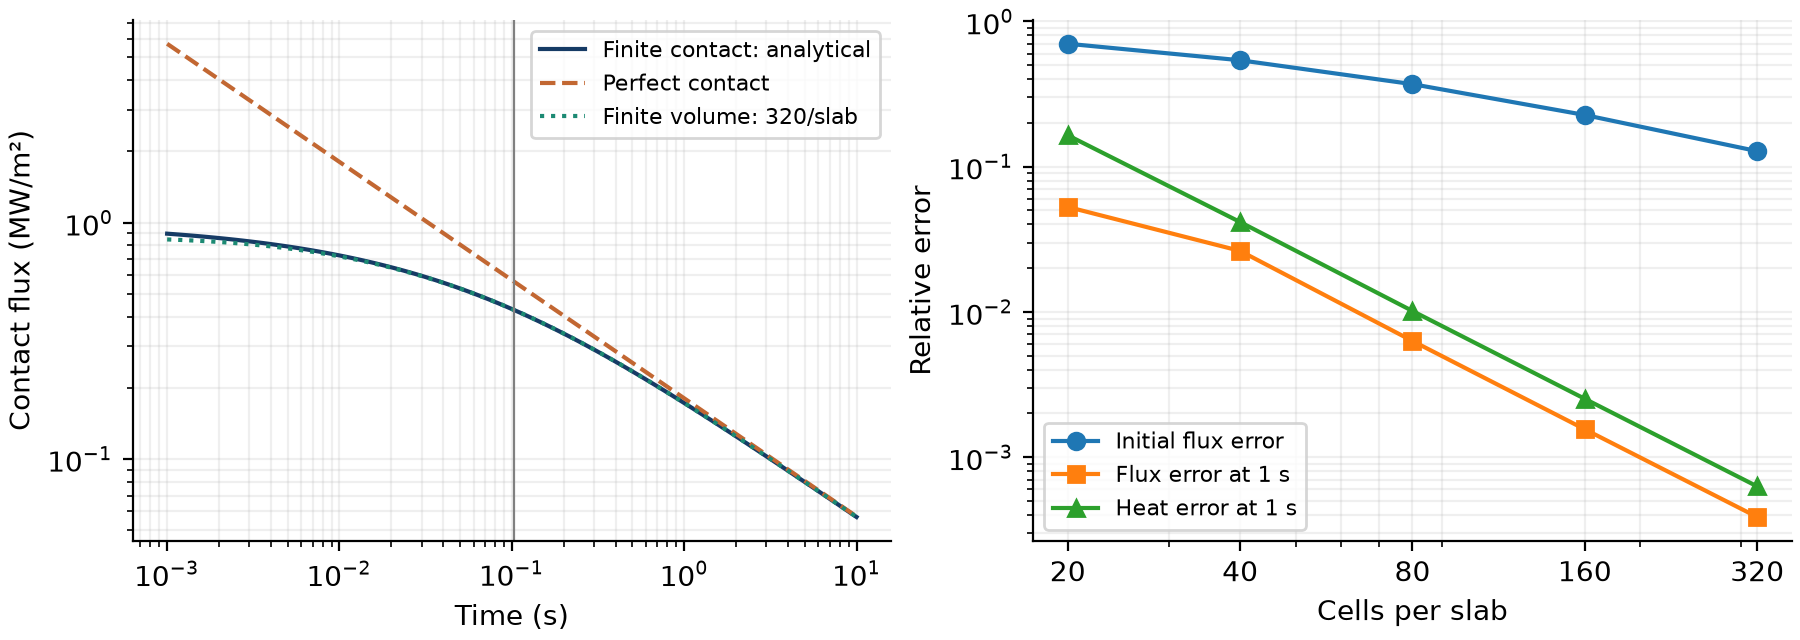
\includegraphics[width=\textwidth]{../results/contact-study.png}
\caption{Left: finite-contact reference and finest finite-volume flux, compared
with perfect contact; the vertical line marks $t_c$. Right: error at the initial
instant and at one second. All plotted data are generated by the project.}
\label{fig:study}
\end{figure}
\begin{table}[ht]
\centering
\begin{tabular}{rrrr}
\toprule
Cells/slab & $q_h(0)/q(0)$ & $E_q(1)$ & $E_Q(1)$ \\
\midrule
20 & 0.29907 & 5.275e-02 & 1.643e-01 \\
40 & 0.46043 & 2.627e-02 & 4.152e-02 \\
80 & 0.63054 & 6.302e-03 & 1.014e-02 \\
160 & 0.77341 & 1.554e-03 & 2.520e-03 \\
320 & 0.87223 & 3.872e-04 & 6.290e-04 \\
\bottomrule
\end{tabular}

\caption{Initial flux ratio and relative one-second errors. $E_q=|q_h/q-1|$
and $E_Q=|Q_h/Q-1|$. Scientific notation is used for errors.}
\label{tab:refine}
\end{table}

The reference values at one second are $q=\num{\ReferenceFlux}$ W/m$^2$ and
$Q=\num{\ReferenceHeat}$ J/m$^2$. Perfect contact predicts
\num{\PerfectExcess}\% more transferred heat at this time. This difference
is a model-assumption effect, not an error of the finite-contact discretization.
The finest flux refinement order at one second is \FinalOrder; the independent
smooth cell-average test gives order \SmoothOrder.

The initial finite-volume flux is exactly determined by the series resistance:
\begin{equation}
 \frac{q_h(0)}{q(0)}=\frac{1}{1+\eta_h},\qquad
 \eta_h=\frac{h_L/(2k_L)+h_R/(2k_R)}{R}. \label{eq:mesh}
\end{equation}
Thus the coarse mesh resolves less than one third of the initial flux, and
even the finest mesh remains below nine tenths (Table~\ref{tab:refine}).
The finest observed positive-time flux error over the recorded interval is
about $5.46\%$; its heat error reaches $7.54\%$. The corresponding one-second
errors are much smaller. A single late observation is consequently insufficient
to certify early contact resolution.

On the recorded local run, the small-chain modal/dense-exponential discrepancy
is \num{\DenseError} K. The maximum energy-balance residual over all contact
histories is \num{\BalanceError} J/m$^2$ (roundoff relative to large sensible
energies). Domain doubling changes the final flux by a relative
\num{\DomainError}; this is below a useful roundoff-level distinction and is
not an estimate accurate to all displayed digits. These diagnostics are stored
in machine-readable form and tested against explicit cross-platform budgets.
\clearpage

\section{Discussion and limitations}
Equation~\eqref{eq:mesh} identifies a practical spatial criterion for measuring
the initial contact law: $\eta_h$ must be small. Requiring an initial relative
flux deficit below a chosen $\epsilon$ implies
$\eta_h<\epsilon/(1-\epsilon)$. This is an initial-state condition, not a
universal bound on every later temperature or heat-transfer error. The declining
contact flux and growing diffusion layers explain why later agreement can look
better than the initial ratio. The refinement table demonstrates this effect
for one deliberately specified pair of materials.

Three error levels remain separate. First, the two-cell solution, dense
exponential and discrete heat/energy identities verify the finite-dimensional
solver. The constant mode is treated analytically, although roundoff leakage
from other computed modes remains. Second, the half-space comparison measures
spatial error together with any finite-domain mismatch; the domain-doubling
check bounds that concern only empirically at the reported final time and
spacing. The homogeneous cosine experiment independently verifies smooth
continuum convergence. Third, none of these calculations validates a real
contact resistance or the assumptions in Eq.~\eqref{eq:pde}.

The model excludes roughness evolution, pressure dependence, thermal expansion,
temperature-dependent properties, latent heat and interfacial heat capacity.
The two synthetic bodies have no asserted material identity. Equal cell counts
and the chosen lengths happen to match the diffusive length ratio, but the
method accepts arbitrary positive cell properties. Extreme floating-point scales,
nearly disconnected chains and very large grids are outside the tested range.
There is no inference of $R$ from noisy data and no measured runtime speedup.

\section{Conclusion and reproducibility}
A late-time flux check can hide an unresolved thermal contact. For this study,
the one-second flux approaches second-order spatial convergence while the
initial deficit follows a first-order half-cell resistance effect. Reporting
both the physical crossover $t_c$ and the mesh ratio $\eta_h$ makes the
distinction explicit. Further work could test temperature-dependent contact
laws or compare with independently measured interface data.

Install with \texttt{python -m pip install -e ".[dev]"}; run
\texttt{contactscale --output results} to regenerate all study data and the
figure. Run \texttt{python -m pytest} for the test suite and execute
\path{scripts/check_results.py} with Python for numerical reproduction.
Build this paper by executing \path{scripts/build_paper.py}; the script accepts
pdfLaTeX or Tectonic, rejects undefined references and overfull boxes, enforces
at most five pages and records source/PDF hashes. CI runs the software on
Windows and Linux and compiles the paper independently. No authorship,
affiliation or peer review is asserted by this manuscript.

\begin{thebibliography}{9}
\bibitem{nist} NIST Digital Library of Mathematical Functions.
Chapter 7, especially \S7.12, asymptotic expansions of the complementary error
function. \url{https://dlmf.nist.gov/7.12}. Accessed 19 October 2026.
\bibitem{erfcx} SciPy contributors. \texttt{scipy.special.erfcx} reference.
\url{https://docs.scipy.org/doc/scipy/reference/generated/scipy.special.erfcx.html}.
Accessed 19 October 2026.
\bibitem{eigh} SciPy contributors. \texttt{scipy.linalg.eigh\_tridiagonal} reference.
\url{https://docs.scipy.org/doc/scipy/reference/generated/scipy.linalg.eigh_tridiagonal.html}.
Accessed 19 October 2026.
\end{thebibliography}
\end{document}
